\section{Introduction}
\label{sec:introduction}

\lipsum[2]

\begin{figure*}
	\centering
	\begin{subfigure}[b]{0.33\textwidth}
		\centering
		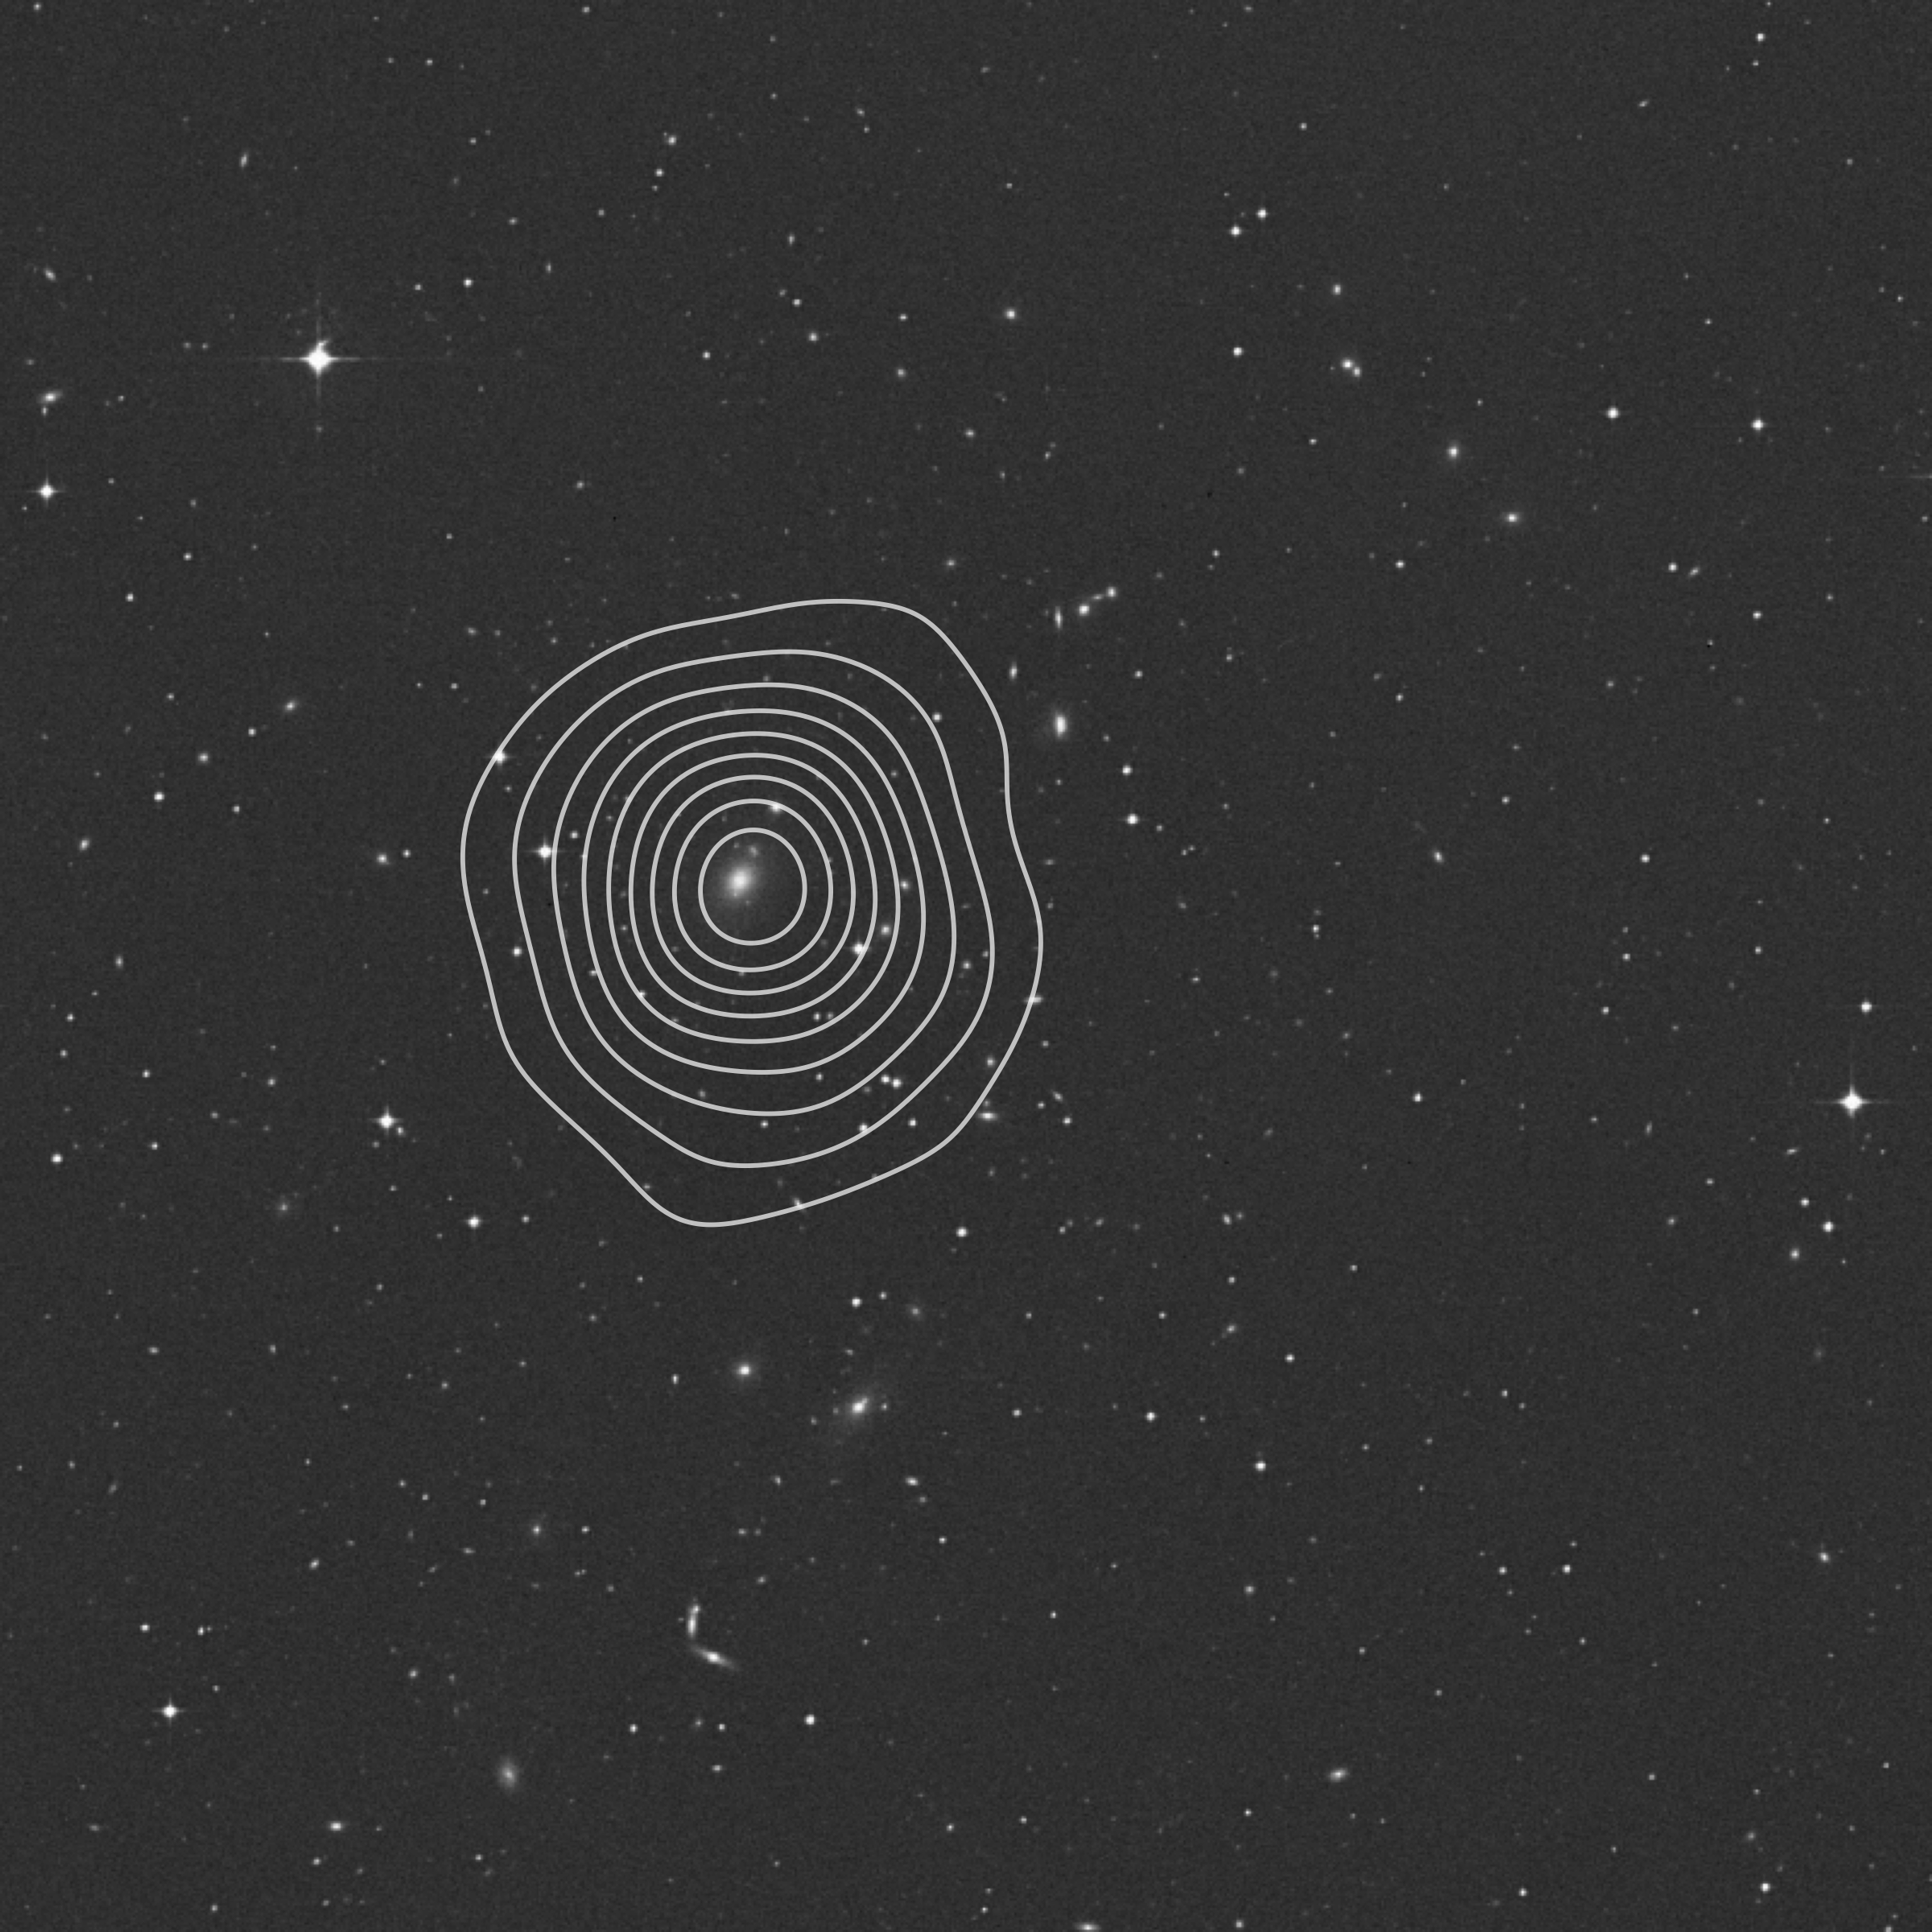
\includegraphics[width=\textwidth]{catalog/ROSAT/RASS-DSS2-A85-overlay.png}
		\caption{Abell 85}
	\end{subfigure}
	\hfill
	\begin{subfigure}[b]{0.33\textwidth}
		\centering
		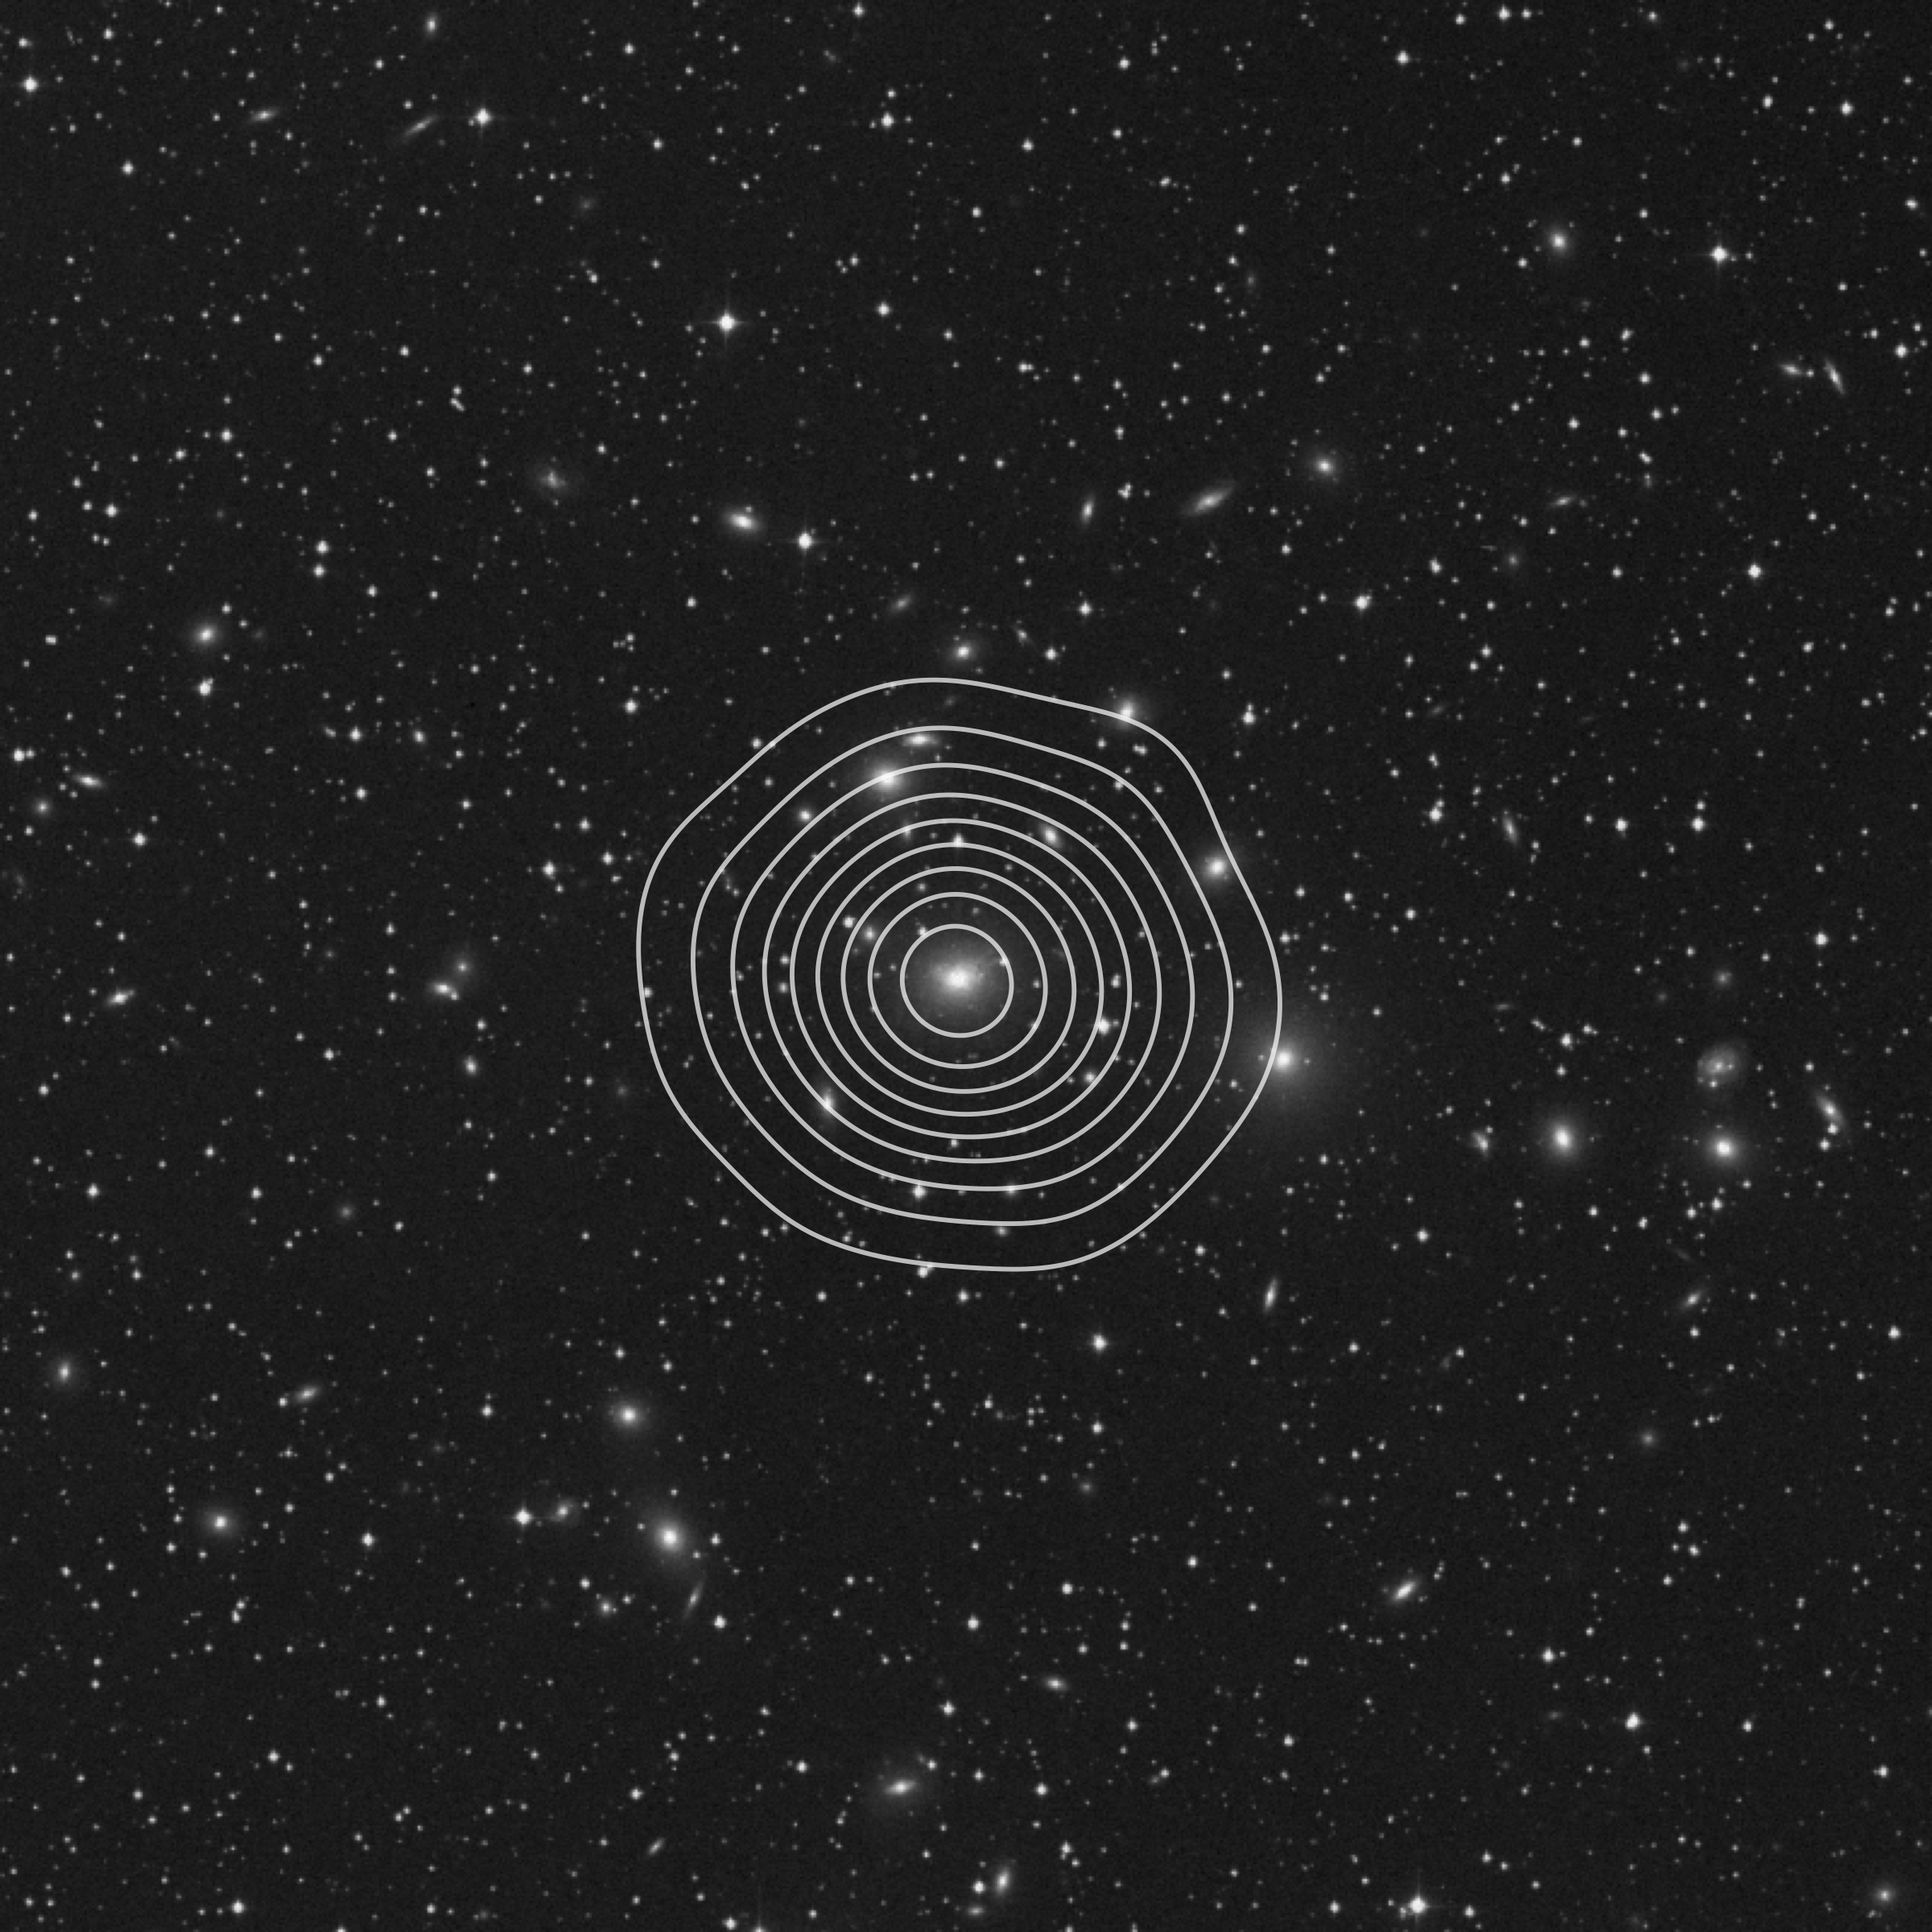
\includegraphics[width=\textwidth]{catalog/ROSAT/RASS-DSS2-A426-overlay.png}
		\caption{Abell 426 (Perseus)}
	\end{subfigure}
	\hfill
	\begin{subfigure}[b]{0.33\textwidth}
		\centering
		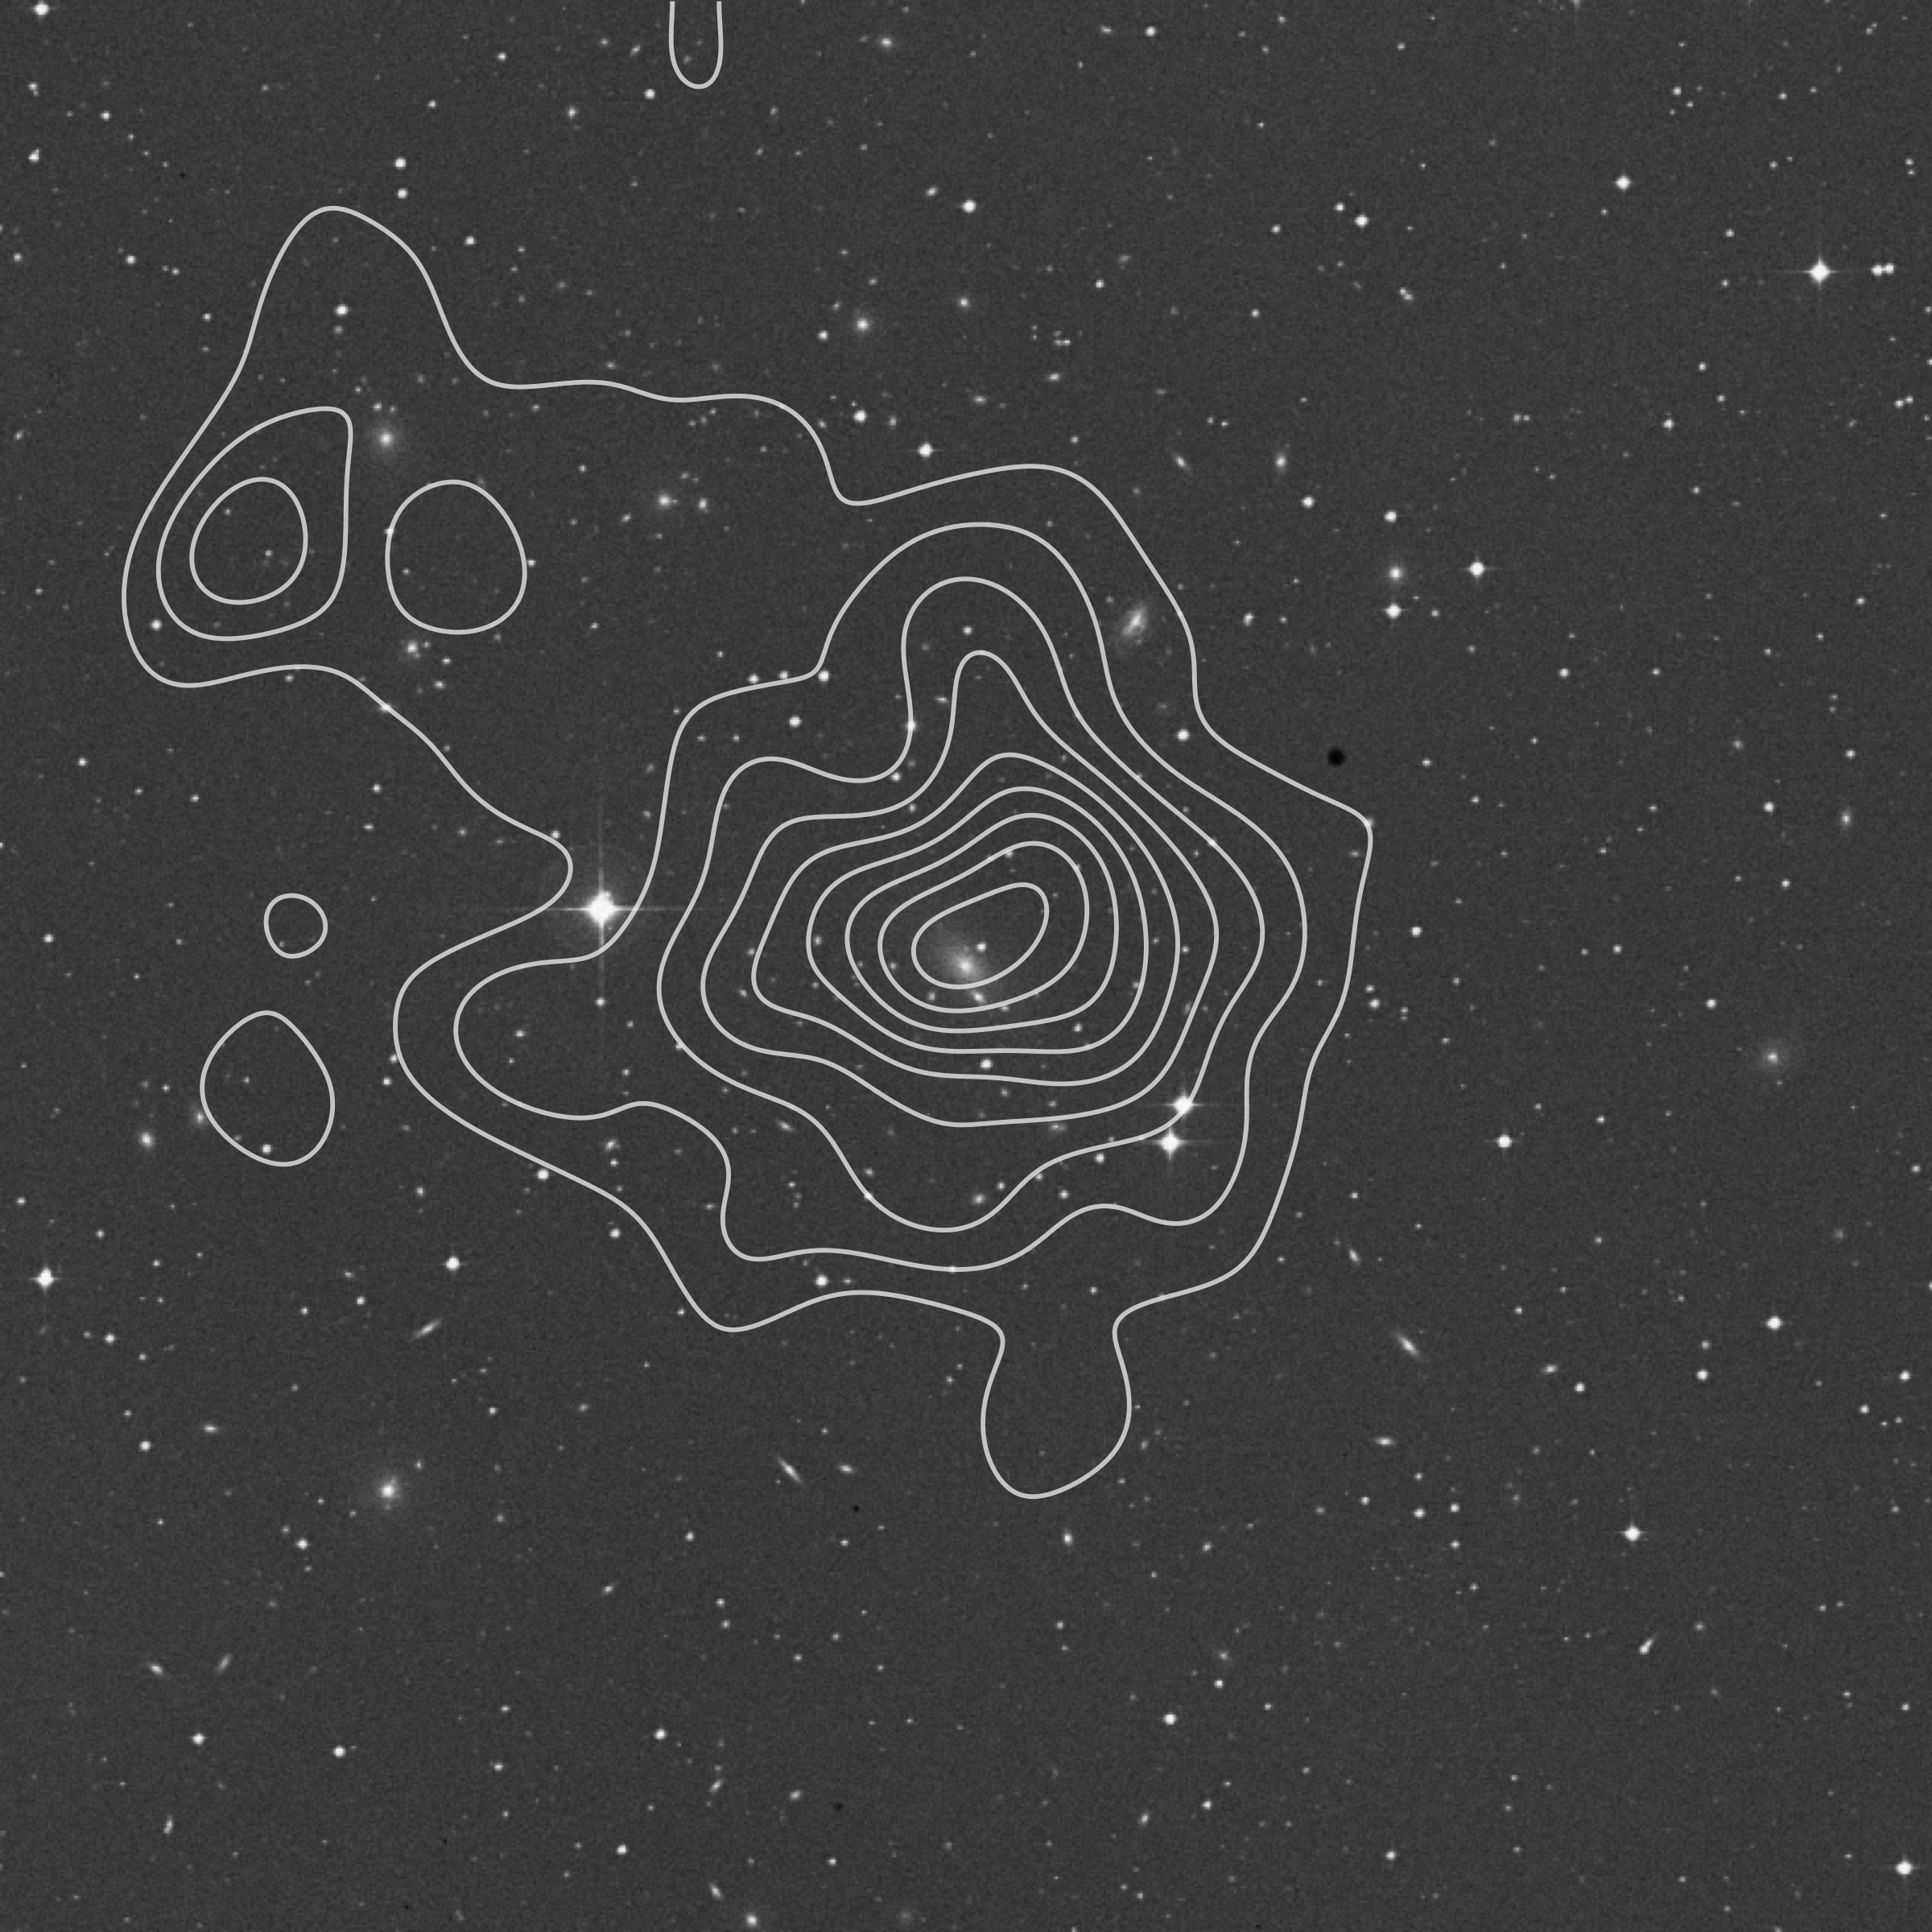
\includegraphics[width=\textwidth]{catalog/ROSAT/RASS-DSS2-A1644-overlay.png}
		\caption{Abell 1644}
	\end{subfigure}

	\vspace{1ex}

	\begin{subfigure}[b]{0.33\textwidth}
		\centering
		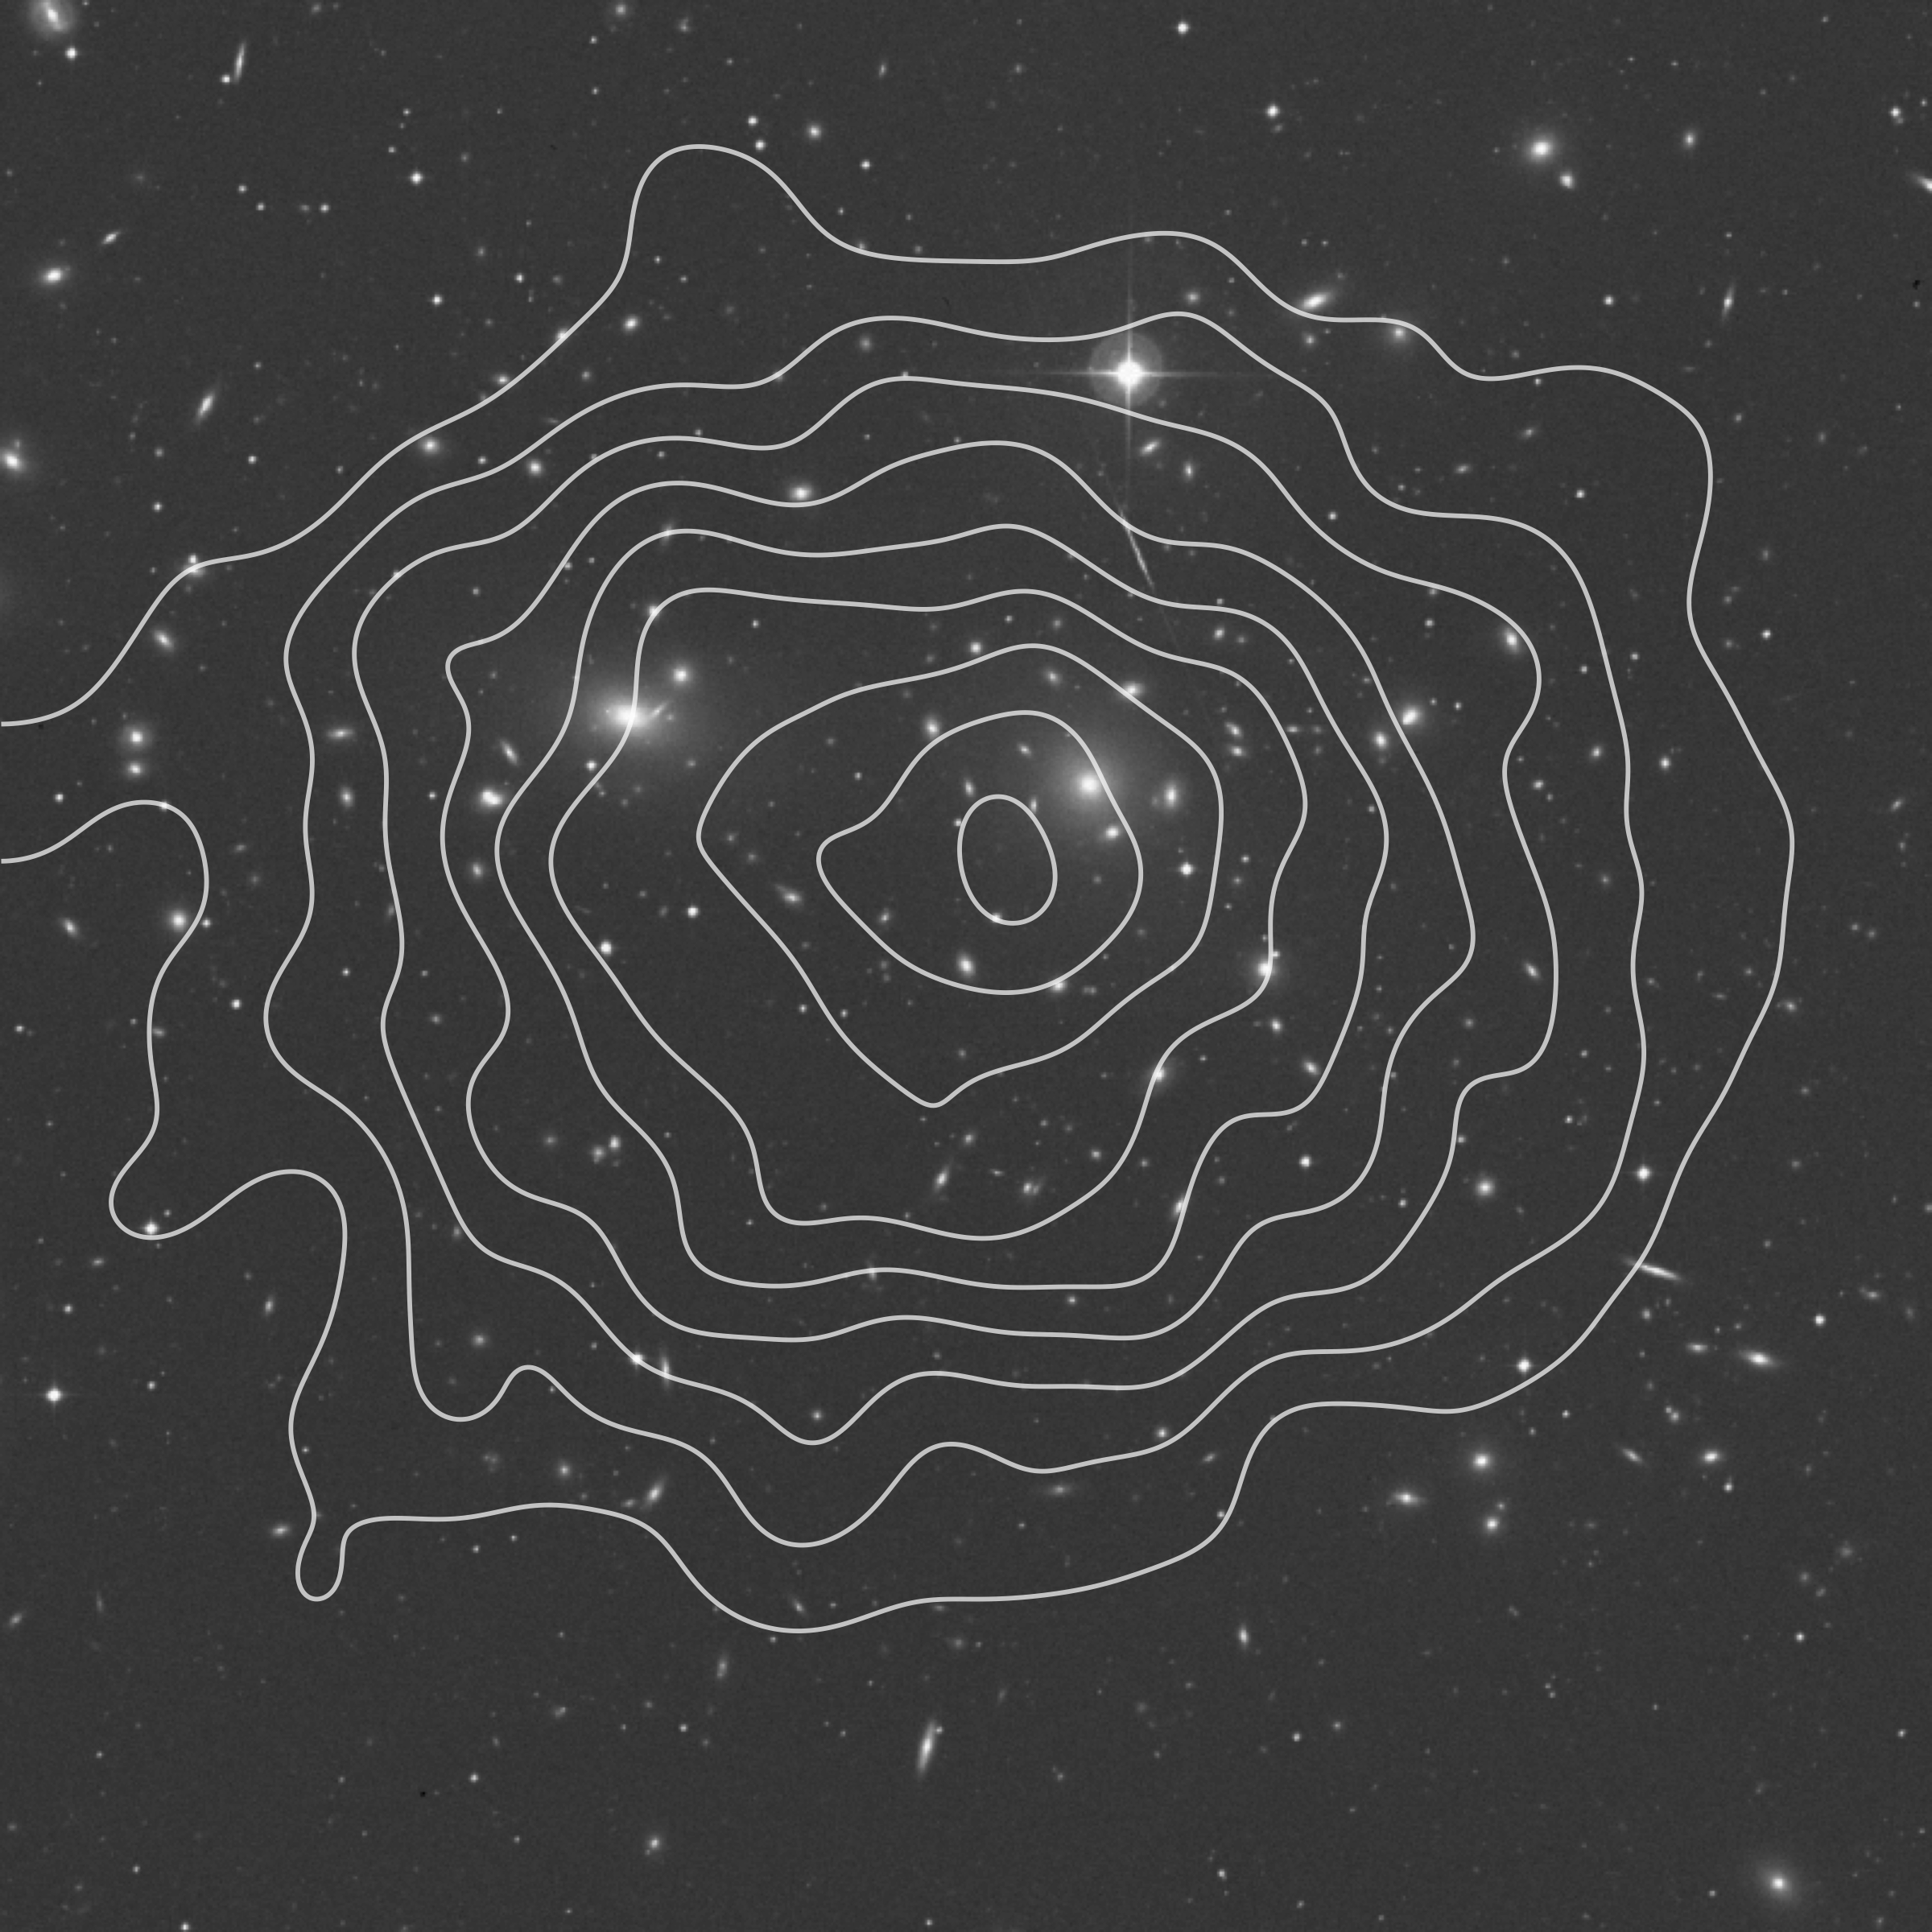
\includegraphics[width=\textwidth]{catalog/ROSAT/RASS-DSS2-A1656-overlay.png}
		\caption{Abell 1656 (Coma)}
	\end{subfigure}
	\hfill
	\begin{subfigure}[b]{0.33\textwidth}
		\centering
		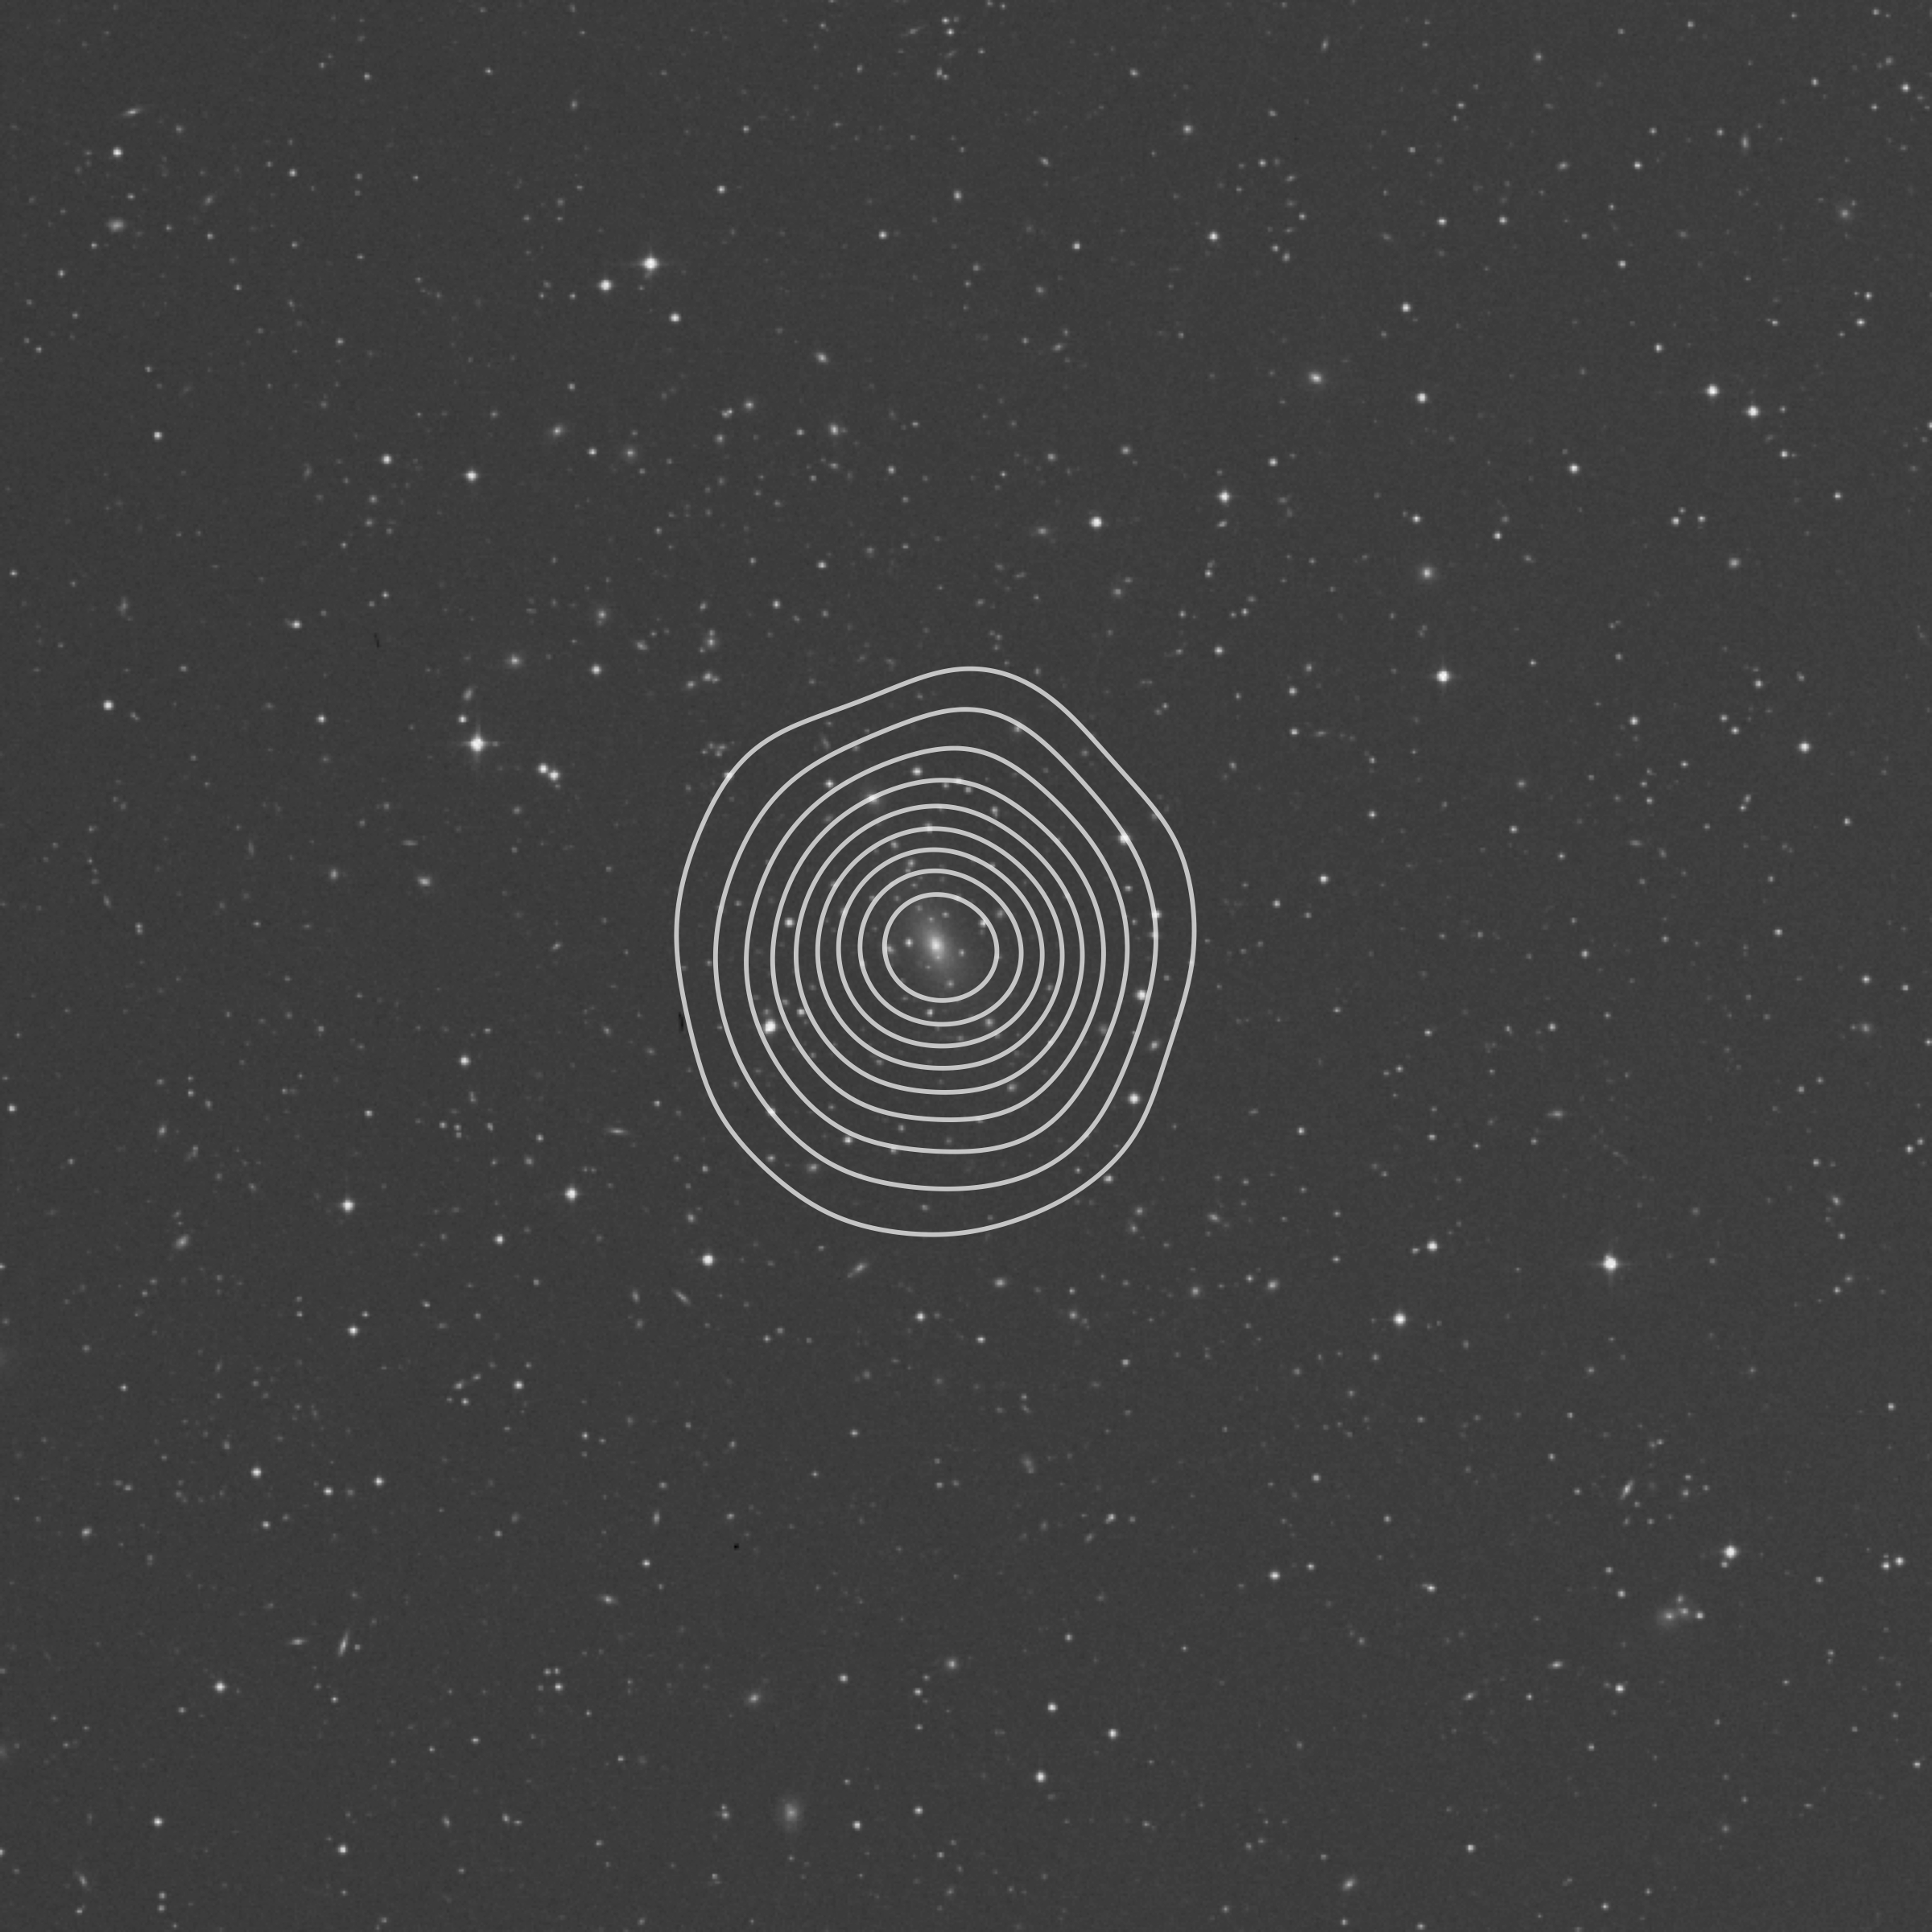
\includegraphics[width=\textwidth]{catalog/ROSAT/RASS-DSS2-A2029-overlay.png}
		\caption{Abell 2029}
	\end{subfigure}
	\hfill
	\begin{subfigure}[b]{0.33\textwidth}
		\centering
		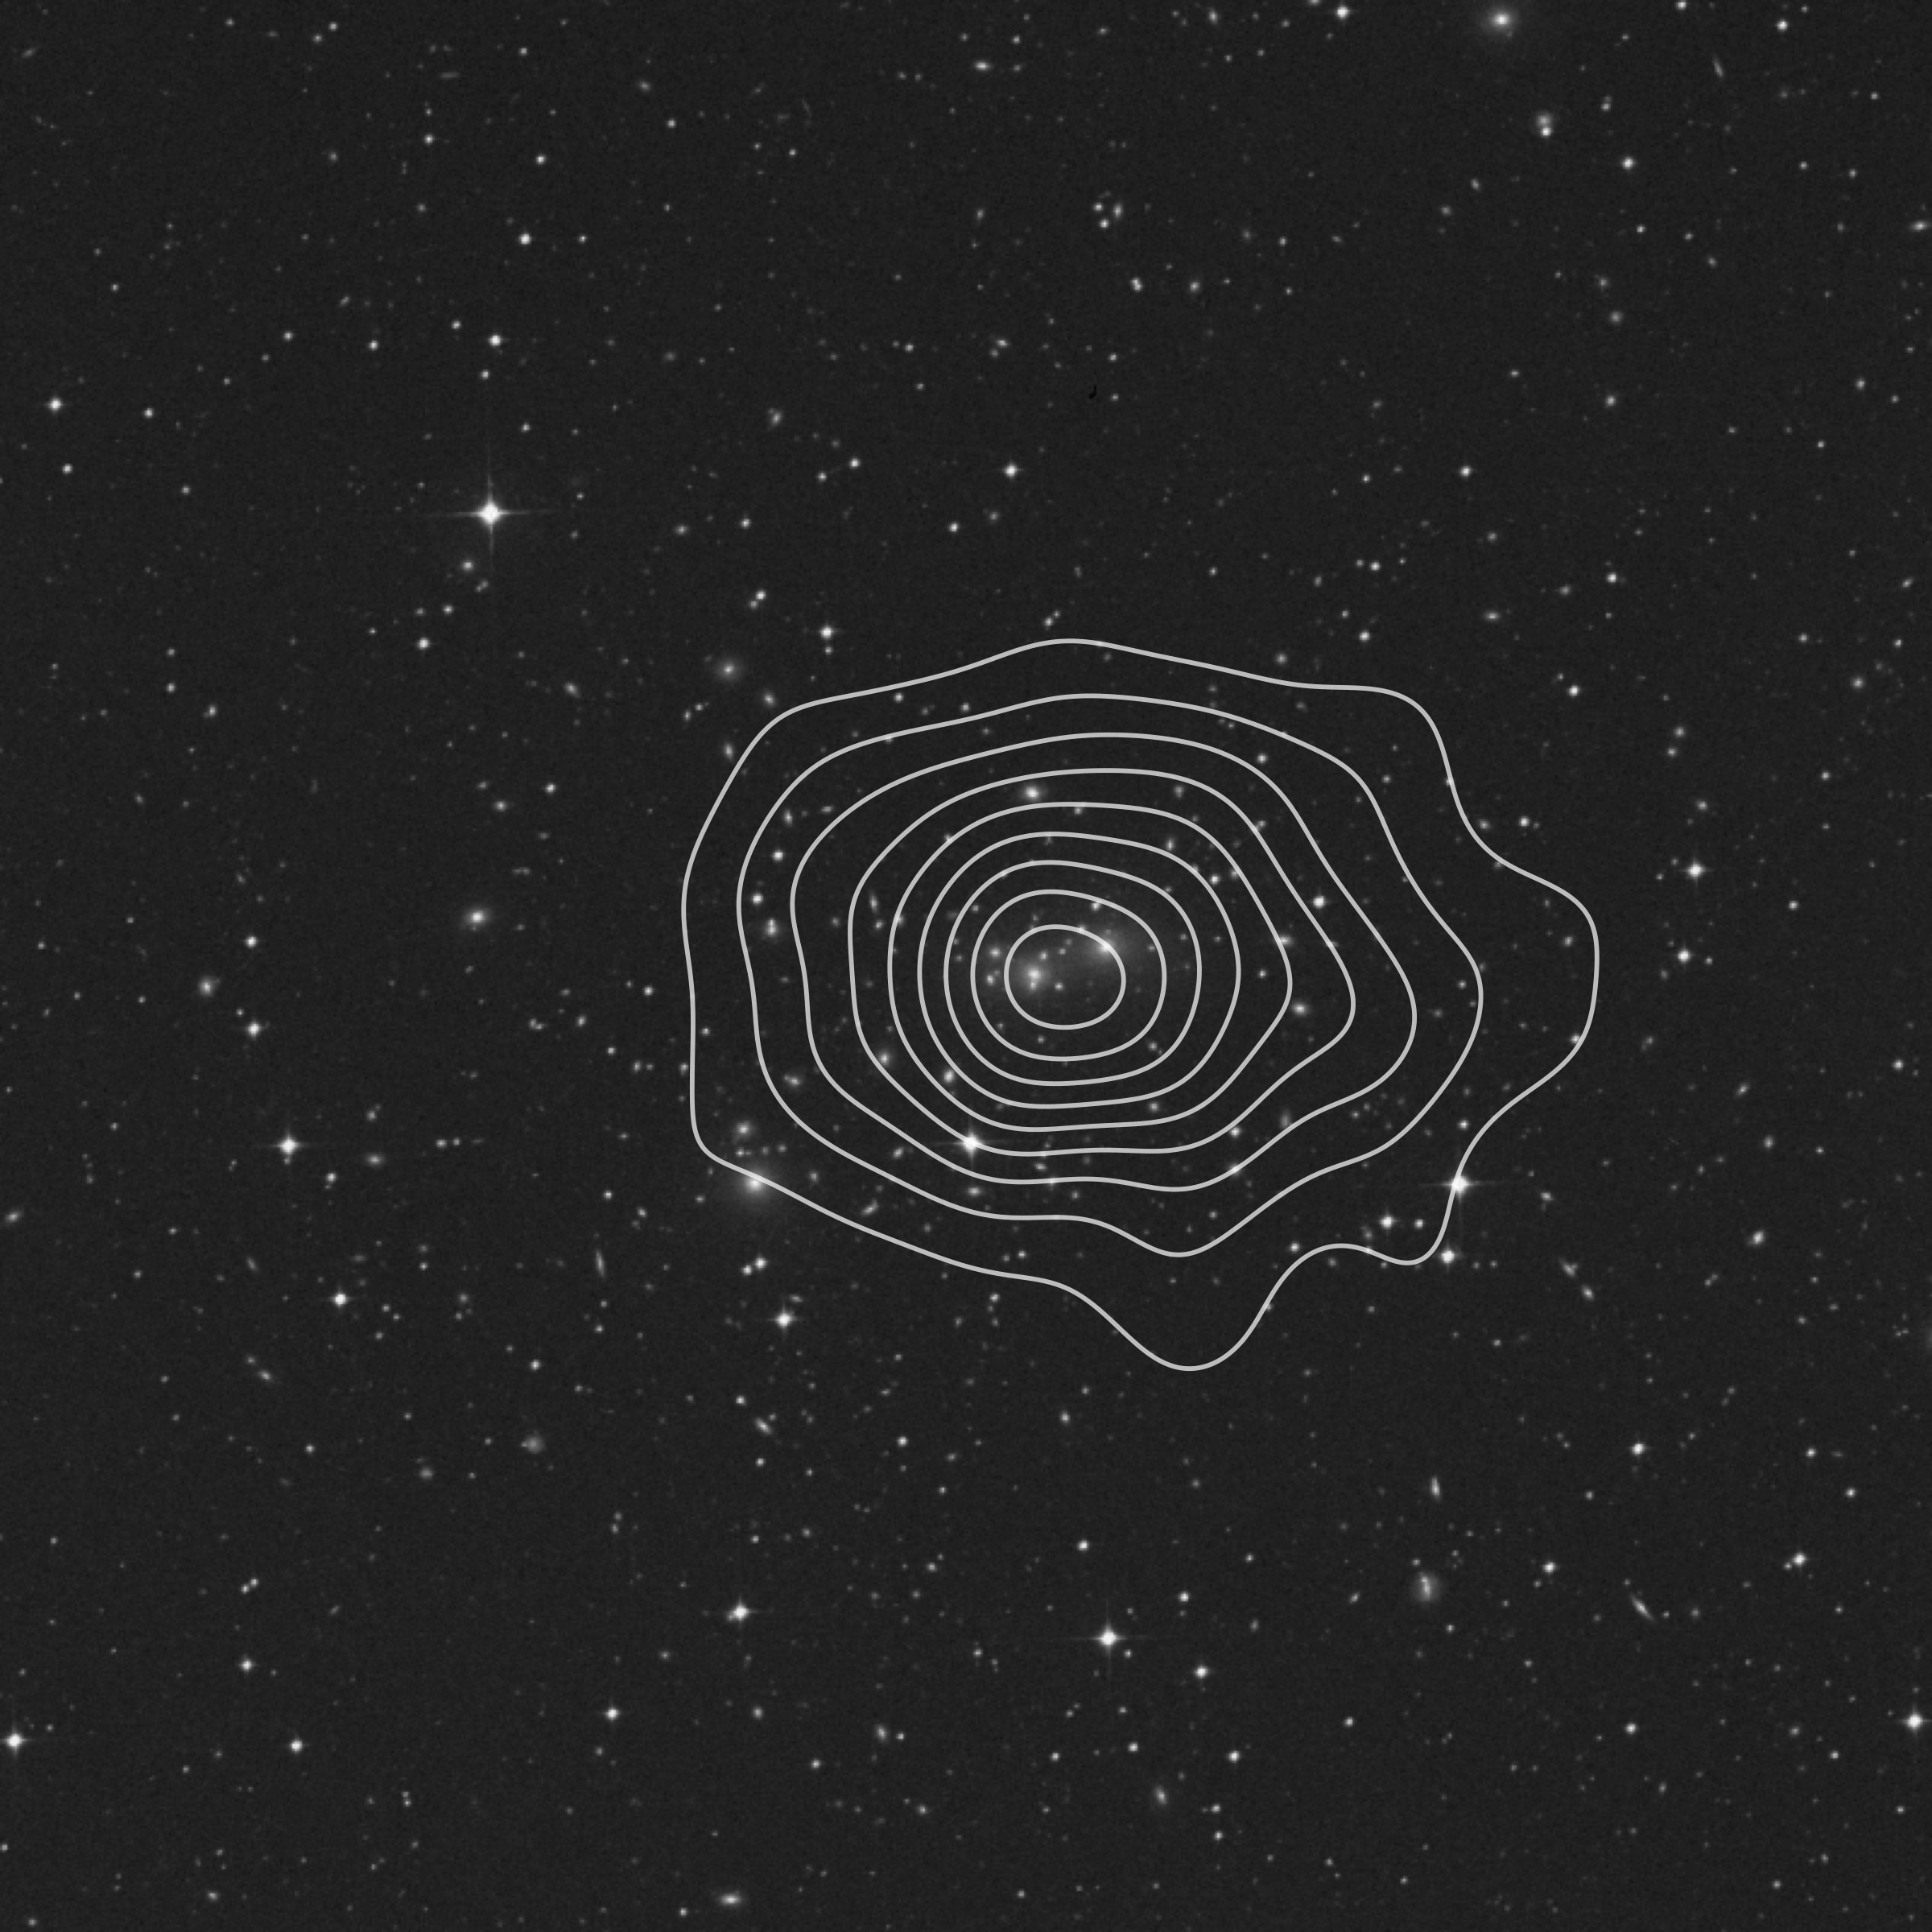
\includegraphics[width=\textwidth]{catalog/ROSAT/RASS-DSS2-A3158-overlay.png}
		\caption{Abell 3158}
	\end{subfigure}
	\caption{Selection of galaxy clusters used as examples in this work. Displayed here
			 are composite overlays of second generation \textit{Digitized Sky Survey} red band
			 images and contours for \textit{ROSAT All Sky Survey (RASS)} broad band count rates
			 \cite{true1982, lask1994}. Both optical and \xray data are stretched using a simple
			 $0.8$ exponent power law. Each frame has a radius of \ang{;15} for its field of view.
			 Refer to \bCref{fig:obs_raw} for raw \textit{ROSAT} counts underlying the contours.}
	\label{fig:obs_overlay}
\end{figure*}
